%%%%%%%%%%%%%%%%%%%%%%%%%%%%%%%%%%%%%%%%%%  不使用 authblk 包制作标题  %%%%%%%%%%%%%%%%%%%%%%%%%%%%%%%%%%%%%%%%%%%%%%
%-------------------------------PPT Title-------------------------------------
\title{13-$\vec k$-空间布点与积分}
%-----------------------------------------------------------------------------
%----------------------------Author & Date------------------------------------

%\author[\textrm{Jun\_Jiang}]{姜\;\;骏\inst{}} %[]{} (optional, use only with lots of authors)
%% - Give the names in the same order as the appear in the paper.
%% - Use the \inst{?} command only if the authors have different
%%   affiliation.
%\institute[BCC]{\inst{}%
\institute[Gain~Strong]{\inst{}%
%\vskip -20pt 北京市计算中心}
\vskip -20pt {\large 格致斯创~科技}}
\date[\today] % (optional, should be abbreviation of conference name)
{%	{\fontsize{6.2pt}{4.2pt}\selectfont{\textcolor{blue}{E-mail:~}\url{jiangjun@bcc.ac.cn}}}
\vskip 45 pt {\fontsize{8.2pt}{6.2pt}\selectfont{%清华大学\;\;物理系% 报告地点
	\vskip 5 pt \textrm{2023.05.27}}}
}

%% - Either use conference name or its abbreviation
%% - Not really information to the audience, more for people (including
%%   yourself) who are reading the slides onlin%%   yourself) who are reading the slides onlin%%   yourself) who are reading the slides onlineee
%%%%%%%%%%%%%%%%%%%%%%%%%%%%%%%%%%%%%%%%%%%%%%%%%%%%%%%%%%%%%%%%%%%%%%%%%%%%%%%%%%%%%%%%%%%%%%%%%%%%%%%%%%%%%%%%%%%%%

\subject{}
% This is only inserted into the PDF information catalog. Can be left
% out.
%\maketitle
\frame
{
%	\frametitle{\fontsize{9.5pt}{5.2pt}\selectfont{\textcolor{orange}{“高通量并发式材料计算算法与软件”年度检查}}}
\titlepage
}
%-----------------------------------------------------------------------------

%------------------------------------------------------------------------------列出全文 outline ---------------------------------------------------------------------------------
\section*{}
\frame[allowframebreaks]
{
  \frametitle{Outline}
%  \frametitle{\textcolor{mycolor}{\secname}}
  \tableofcontents%[current,currentsection,currentsubsection]
}
%%在每个section之前列出全部Outline
%%类似的在每个subsection之前列出全部Outline是\AtBeginSubsection[]
%\AtBeginSection[]
%{
%  \frame<handout:0>%[allowframebreaks]
%  {
%    \frametitle{Outline}
%%全部Outline中,本部分加亮
%    \tableofcontents[current,currentsection]
%  }
%}

%-----------------------------------------------PPT main Body------------------------------------------------------------------------------------
\small
%\section{\rm{VASP~}软件中\rm{PAW~}计算的实现}
%\frame
%
%	\frametitle{\textrm{VASP}计算的特色}
%	相比于与普通的第一原理计算软件,\textrm{VASP}很好地平衡了计算效率和精度的问题,总的来说,\textrm{VASP}主要通过这几个特色保证了计算的高效能
%	\begin{itemize}
%	     \item 迭代与优化算法的多样性\\
%		     本质上电荷密度迭代 \textrm{\&\&} 体系总能量优化是相同的优化问题,采用了类似的算法\upcite{CMS6-15_1996,PRB54-11169_1996}:\\
%			\textcolor{blue}{\textrm{Pseudo-Newton、Conjugate-Gradient、Broyden~mix、damping-factor、RMM-DIIS}}
%	     \item 尽可能采用局域基(原子轨道基)函数:~\\
%		     \textcolor{blue}{\textrm{LREAL}}=\textcolor{red}{\textrm{.TRUE.}}\\
%			优化的投影函数也尽可能在实空间表示
%	     \item \textrm{PAW}原子数据集:\textcolor{blue}{优异的赝势}\upcite{PRB59-1758_1999}
%	\end{itemize}
%}
\section{$\vec k$~空间布点与积分}
\frame
{
	\frametitle{$\vec k$~空间布点与\textrm{Fermi~}面的确定}
\begin{figure}[h!]
\centering
\hspace*{-0.35in}
\subfigure[\textrm{Brillouin Zone of Cubic lattice}]{
\label{Brillouin_Zone_Cubic-2}
\vspace*{-0.50in}
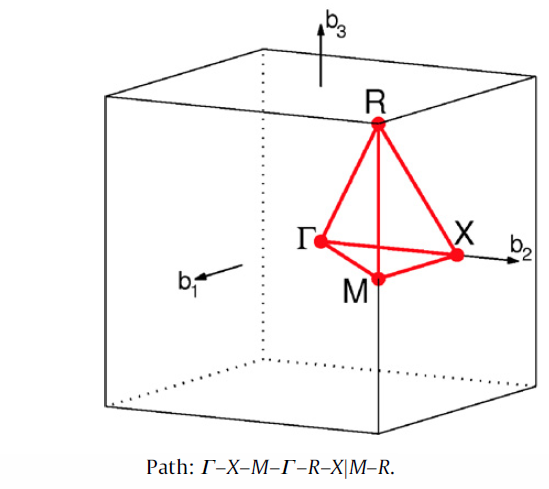
\includegraphics[height=2.10in,width=2.00in,viewport=90 0 550 500,clip]{Figures/Brillouin-Zone_CUB.png}}
\subfigure[\textrm{Band Structure of SrSnO$_3$}]{
\label{Band_Gap_SrSnO3-2}
\vspace*{-0.50in}
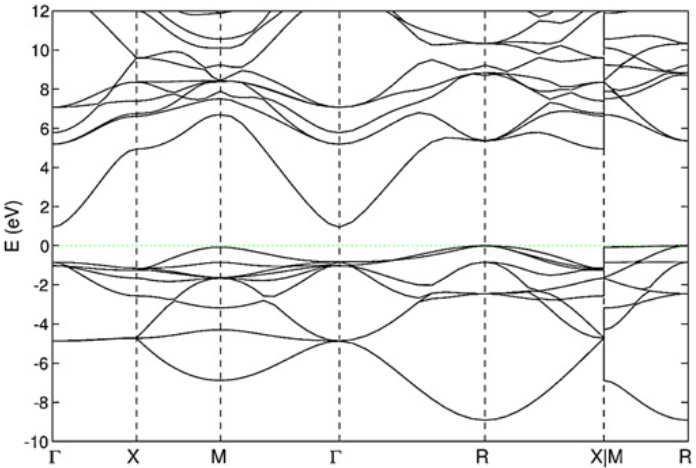
\includegraphics[height=2.10in,width=1.95in,viewport=0 0 710 550,clip]{Figures/Band-Struct_SrSnO3.png}}
\label{Band_Gap_CUB_SrSnO3}
\end{figure}
在固体能带理论中,\textcolor{blue}{能量色散关系$\varepsilon(\vec k)$}~表示能量在倒空间中分布,其中量子数$\vec k$~(晶体动量)描述平移对称性
%\textcolor{blue}{能带图表示能量在\textrm{Brillouin-zone~}特定方向的色散关系}
}

\frame
{
	\frametitle{$\vec k$~空间布点与\textrm{Fermi~}面的确定}
\begin{figure}[h!]
\centering
%\hspace*{-10pt}
\vspace*{-0.3in}
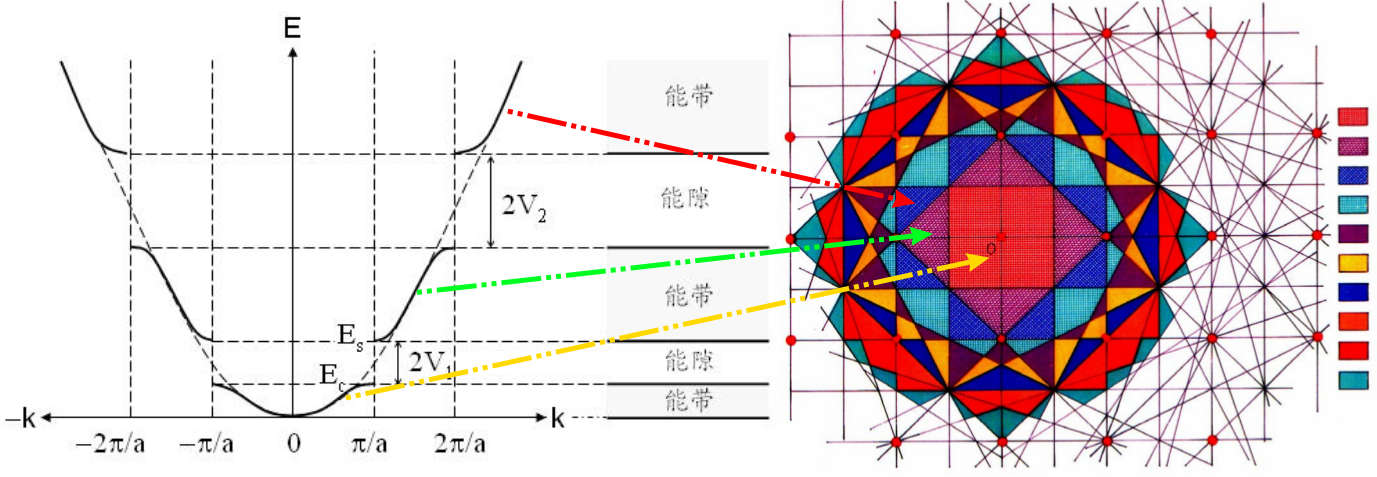
\includegraphics[height=1.5in,width=4.1in,viewport=0 5 1400 500,clip]{Figures/Brillouin-Band.png}
\caption{\tiny \textrm{The relation between unfolded-Band and the Brillouin-zone.}}%
\label{Brillouin-Band}
\end{figure} 
周期体系的\textrm{Fermi~}能级和\textrm{Fermi~}面的确定:\\
\begin{displaymath}
	\left\{
	\begin{aligned}
		&\mbox{\textcolor{red}{导体:~}}&\mbox{\textcolor{blue}{价电子在\textrm{Brillouin-zone~}部分填充}}\\
		&\mbox{\textcolor{red}{半导体-绝缘体:~}}&\mbox{\textcolor{blue}{价电子在\textrm{Brillouin-zone~}完全填充}}
	\end{aligned}\right.
\end{displaymath}
}

\frame
{
	\frametitle{$\vec k$~空间布点与\textrm{Fermi~}面的确定}
\begin{figure}[h!]
\centering
%\hspace*{-10pt}
\vspace*{-0.15in}
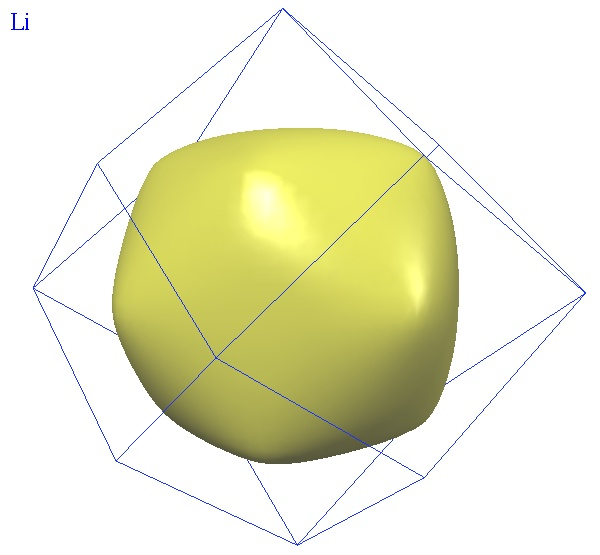
\includegraphics[height=1.2in,width=1.3in,viewport=0 0 110 100,clip]{Figures/FS-Li.jpg}
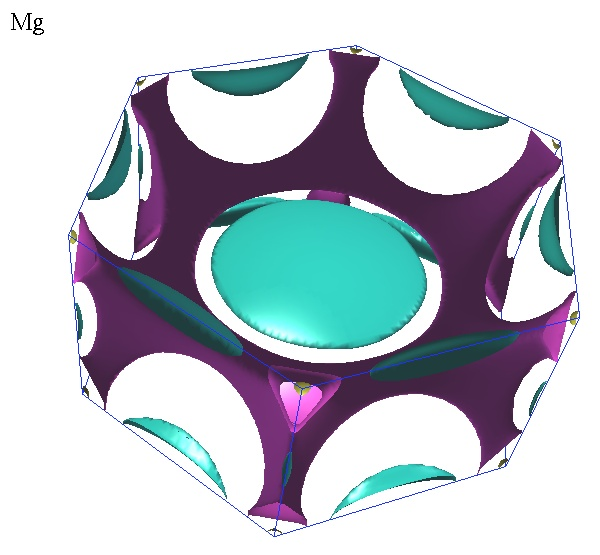
\includegraphics[height=1.2in,width=1.3in,viewport=0 0 110 100,clip]{Figures/FS-Mg.jpg}
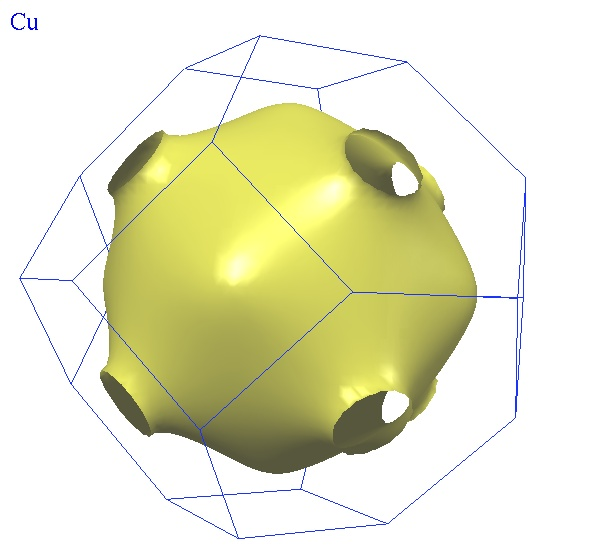
\includegraphics[height=1.2in,width=1.3in,viewport=0 0 110 100,clip]{Figures/FS-Cu.jpg}
\caption{\tiny \textrm{The Fermi-surface of Li, Mg, Cu in the first Brillouin-zone.}}%
\label{Brillouin-Band-Fermi}
\end{figure} 
\textcolor{blue}{\textrm{Fermi~}面的形状}:\\
\textcolor{red}{最高占据能带折叠到第一\textrm{Brillouin-zone~}围成的区域}

\vspace{10pt}
要确定\textrm{Fermi~}面的精细结构,\underline{\textcolor{red}{特别是对于金属和导体体系}},必须在整个\textrm{Brillouin-zone~}取足够多的采样点
}

\frame
{
\frametitle{$\vec k$~空间积分与物理量计算}
与\textrm{Fermi~}面的确定类似,周期体系中所有单粒子期望值可表示为整个\textrm{Brillouin-zone~}内占据态的矩阵元的积分\\

一般地,如果已知\textrm{Brillouin-zone~}某点$\vec k$~的能带指标为$n$的波函数本征态$\Psi_n(\vec k)$~和本征值$\epsilon_n(\vec k)$,算符$\mathbf{X}$~的期望值$\langle X \rangle$是矩阵元
\begin{displaymath}
	X_n(\vec k)=\langle\Psi_n(\vec k)|\mathbf{X}|\Psi_n(\vec k)\rangle 
\end{displaymath}
\textcolor{blue}{在倒空间全部占据能带的求和}
\begin{displaymath}
	\langle X\rangle=\dfrac1{\sqrt V_G}\sum_n\int_{V_G}\mathrm{d}^3kX_n(\vec k)f(\varepsilon_n(\vec k))
\end{displaymath}
其中$V_G$是第一\textrm{Brillouin-zone}体积,$f(\varepsilon)$~是占据分布函数

实际计算中,\textrm{Brillouin-zone~}的$\vec k$~点数是有限的
\begin{displaymath}
	\langle X\rangle=\sum_{j,n}X_n(\vec k_j)w_n^{\vec k_j}
\end{displaymath} 
\textcolor{blue}{$\vec k$~点数目决定了电子结构和物理量的的精度与计算量}
}

\frame
{
\frametitle{$\vec k$~空间布点方案}
\begin{enumerate}
	\item \textcolor{red}{简单分布函数}\\
		\begin{itemize}
			\item 
				\begin{figure}[h!]
					\begin{minipage}[t]{0.40\linewidth}
						\textrm{Fermi-Dirac~}分布函数$$f(\varepsilon)=\dfrac1{\mathrm{e}^{(\varepsilon-\mu)/kT}+1}$$ 
						其中$\mu$是化学势,$k$~是\textrm{Boltzmann}常数,$T$是温度参数
					\end{minipage}
				\hfill
					\begin{minipage}[t]{0.55\linewidth}
					\centering
					\vspace*{-0.35in}
					\hspace*{-0.5in}
					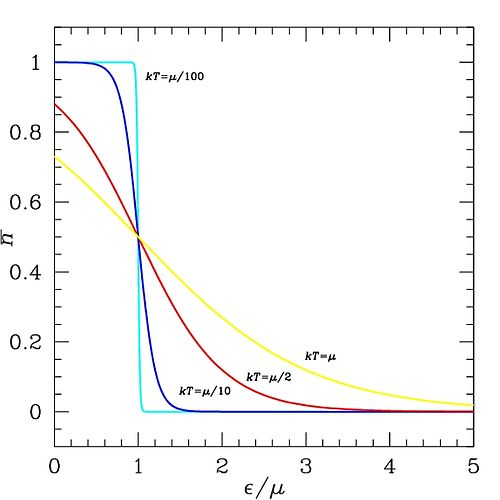
\includegraphics[height=1.0in,width=1.25in,viewport=0 0 530 500,clip]{Figures/Fermi-Dirac-distribution.jpg}
					\caption{\textrm{The Fermi-Dirac Distribution.}}%
					\label{Fermi-Dirac-distribution}
					\end{minipage}
					%\hspace*{-10pt}
				\end{figure} 
			\item 
				\begin{figure}[h!]
					\begin{minipage}[t]{0.40\linewidth}
						\textrm{Gaussian~}分布函数$$f(\varepsilon)=\dfrac1{\sigma\sqrt{2\pi}}\mathrm{e}^{-\frac{(\varepsilon-\mu)^2}{2\sigma^2}}$$
						其中$\mu$是化学势,$\sigma$是展宽参数
					\end{minipage}
				\hfill
					\begin{minipage}[t]{0.55\linewidth}
					\centering
					\vspace*{-0.35in}
					\hspace*{-0.5in}
					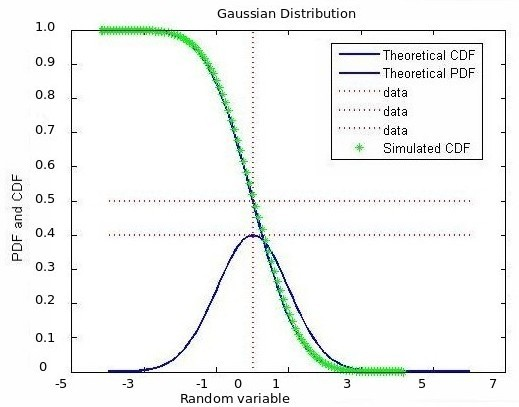
\includegraphics[height=1.0in,width=1.25in,viewport=0 0 530 500,clip]{Figures/Gaussian-distribution.jpg}
					\caption{\tiny \textrm{The Gaussian Distribution.}}%
					\label{Gaussian-distribution}
					\end{minipage}
					%\hspace*{-10pt}
				\end{figure} 
%			\item \textrm{Lorentz~}分布函数$$L(x)=\frac1{\pi}\frac{\frac12\Gamma}{(x-x_0)^2+\left(\frac12\Gamma\right)^2}$$
%				这里$x_0$是中心,$\Gamma$是展宽参数
		\end{itemize}
\end{enumerate}
}

\frame
{
\frametitle{$\vec k$~空间布点方案}
\begin{enumerate}
	\setcounter{enumi}{1}
\setlength{\itemsep}{10pt}
	\item \textcolor{red}{特殊点方法\textrm{(Special-point scheme)}}\\这是一种相对高效的积分方法,通过选取少量有代表性的$\vec k$~点,即可获得较高的计算精度,这些$\vec k$~点被称为“平均值点”或“特殊点”\\特殊点方法对导体的收敛性较差
	\item \textcolor{red}{四面体方法\textrm{(Tetrahedron schemen)}}\\这是一种线性插值方法,将\textrm{Brillouin-zone~}用体积相等的四面体填充,在每个四面体内部,被积函数$X_n(\vec k_j)$和能量$\varepsilon_n^{\vec k_j}$都随$\vec k$~点线性变化\\一般来说,四面体方法对金属和导体的\textrm{Fermi~}面确定更可靠
\end{enumerate}
\textcolor{blue}{如何方便地确定每个$\vec k$~点的积分权重$w_n^{\vec k_i}$,精确、高效地完成\textrm{Brillouin-zone~}积分是$\vec k$~空间布点方案的主要研究内容}
}

\subsection{特殊点布点与积分方法}
\frame
{
	\frametitle{特殊点布点方案}
%如果采用一般的\textrm{Brillouin-zone~}内均匀选取$\vec k$~点的方法,为得到精确的结果,$\vec k$~点的密度必须非常大,从而导致计算量非常大,计算效率低下。因此需要寻求一种高效的积分方法。
	特殊点方法通过少量$\vec k$~点计算取得较高的精度,这些$\vec k$~点称为“平均值点”\upcite{PRB7-5212_1973}或“特殊点”\upcite{PRB8-5747_1973}。
	
	\textrm{Chadi}和\textrm{Cohen}最早提出特殊点方法的数学基础:\\
	考虑任意平滑函数$g(\vec k)$,可以展开为\textrm{Fourier}~级数之和
	$$g(\vec k)=f_0+\sum_{m=1}^{\infty}g_m\mathrm{e}^{\mathrm{i}\vec k\cdot\vec R_m}$$
\begin{figure}[h!]
\begin{minipage}[t]{0.55\linewidth}
	与$g(\vec k)$~对应的具有体系全部对称性的函数$f(\vec k)$,满足
	$$f(\mathbf{T}\vec k)=f(\vec k)\quad\forall\mathbf{T}\in\{\mathbf{G}\}$$
	因此可将$f(\vec k)$用$g(\vec k)$展开
	$$f(\vec k)=\dfrac1{n_{\mathbf{T}}}\sum\limits_ig(\mathbf{T}_i\vec k)$$
\end{minipage}
\hfill
\begin{minipage}[t]{0.42\linewidth}
\centering
\vspace*{-0.5in}
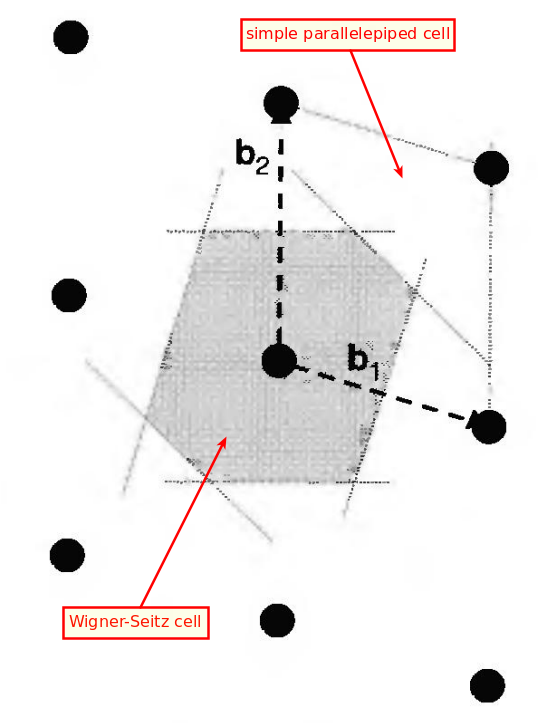
\includegraphics[height=1.8in,width=1.25in,viewport=20 20 530 800,clip]{Figures/Reciprocal-WS.png}
\caption{\tiny \textrm{The Wigner-Seitz Cell (Voronoi polyhedron) in the Brillouin-zone.}}%
\label{Reciprocal-WS}
\end{minipage}
%\hspace*{-10pt}
\end{figure} 
}

\frame
{
	\frametitle{特殊点布点方案}
	$f(\vec k)$可以写成
	$$f(\vec k)=f_0+\sum_{m=1}^{\infty}f_mA_m(\vec k)$$其中
	$$A_m(\vec k)=\sum_{|\vec R|=C_m}\mathrm{e}^{\mathrm{i}\vec k\cdot\vec R}\quad m=1,2,3,\cdots$$
	求和遍历所有对称操作群$\{\mathbf{T}\}$关联的等价矢量$\vec R$,因此$A_m(\vec k)$是实函数,满足
	\begin{displaymath}
		\begin{aligned}
			&\dfrac{V_G}{(2\pi)^3}\int_{\mathrm{BZ}}A_m(\vec k)\mathrm{d}\vec k=0\quad m=1,2,3,\cdots\\
			&\dfrac{V_G}{(2\pi)^3}\int_{\mathrm{BZ}}A_m(\vec k)A_n(\vec k)\mathrm{d}\vec k=N_n\delta_{nm}\quad m=1,2,3,\cdots\\
			&A_m(\mathbf{T}\vec k)=A_m(\vec k)
		\end{aligned}
	\end{displaymath}
}

\frame
{
	\frametitle{特殊点布点方案}
	令$A_0(\vec k)=1$,对函数$f(\vec k)$~在整个\textrm{Brillouin-zone}求平均有
	$$\bar f=\dfrac{V_G}{(2\pi)^3}\int_{\mathrm{BZ}}f(\vec k)\mathrm{d}\vec k=f_0$$
	同样地,函数$g(\vec k)$在\textrm{Brillouin-zone}的积分也是$f_0$

	结论:~\textcolor{red}{可通过选取优化的少量$\vec k$点求和计算平均值}\\如果存在一个$\vec k_0$点满足\textcolor{blue}{
	$$A_m(\vec k_0)=0\quad m=1,2,3,\dots,N$$}
	如果$N\rightarrow\infty$,则有$\bar f=f_0=f(\vec k_0)$精确成立,实际上这样的$\vec k_0$并不存在
\begin{figure}[h!]
\centering
%\hspace*{-10pt}
\vspace*{-0.2in}
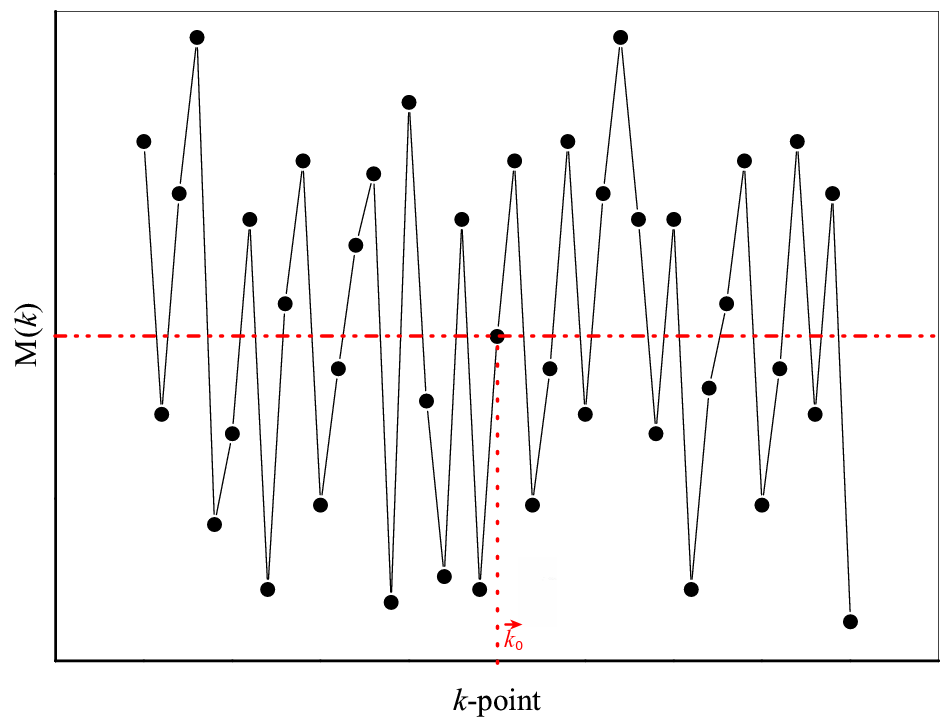
\includegraphics[height=1.1in,width=1.3in,viewport=5 0 960 750,clip]{Figures/Brillouin-k.png}
\caption{\tiny \textrm{The mean value and the $\vec k$-point.}}%
\label{Brillouin-k}
\end{figure} 
}

\frame
{
	\frametitle{特殊点布点方案}
	当$\vec k$-点数目$N$很大时,一般找到单个$\vec k_0$~点不容易,而选择满足一定条件的$\vec k$~点集合$\{\vec k\}$,利用这些$\vec k$~点加权平均计算$f_0$:\\
	假设有如下$\vec k_i$,权重为$\alpha_i$,并满足
	{\fontsize{9.0pt}{3.9pt}\selectfont{\begin{equation}
		\begin{aligned}
			&\sum_{i=1}^n\alpha_iA_m(\vec k_i)=0\quad m=1,2,3,\cdots,N\\
			&\sum_{i=1}^n\alpha_i=1
		\end{aligned}
		\label{eq:Chadi-Cohen}
	\end{equation}}}
	函数$f(\vec k)$在\textrm{Brillouin-zone}的积分值$f_0$可以表示为$$f_0\approx\sum_{i=1}^n\alpha_if(\vec k_i)$$
	\textcolor{blue}{对$\vec k$~点的选择,要求满足}
	\begin{enumerate}
		\item 集合$\{\vec k_i\}$中的$\vec k$~点数目尽可能少
		\item $\vec k_i$在$N$~尽可能大的条件下满足式\eqref{eq:Chadi-Cohen}
	\end{enumerate}
}

\frame
{
	\frametitle{\textrm{Chadi-Cohen}布点方案}
	\textrm{Chadi}和\textrm{Cohen}提出一套可以得到特殊$\vec k$~点的方法:
	\begin{itemize}
		\item \textcolor{blue}{确定两个特殊$\vec k$~点$\vec k_1$和$\vec k_2$}\\
		$\{N_1\}$(对应于$\vec k_1$)和$\{\vec N_2\}$(对应于$\vec k_2$)的情况下满足$$A_m(\vec k)=0$$
	\item \textcolor{blue}{由$\vec k_1$~和$\vec k_2$~确定一套新的$\vec k$~点集合}$$\vec k_i=\vec k_1+\mathbf{T}_i\vec k_2$$
			$\vec k_i$在条件$\vec k_i\in\{N_1\}\cup\{N_2\}$下仍然满足式\eqref{eq:Chadi-Cohen}
		\item \textcolor{blue}{确定$\vec k_i$的权重$\alpha_i$}
			$$\alpha_i=\dfrac{\alpha_i}{\sum\limits_jn_j}$$
	\end{itemize}
	重复上述过程,可以到一些列的特殊$\vec k$~点\\考虑体系对称性,集合$\{\vec k\}$~中的$\vec k$~点数目可以减少
}

\frame
{
	\frametitle{\textrm{Monkhorst-Pack}布点方案}
	\begin{itemize}
		\item \textrm{Chadi-Cohen}方案非常巧妙,但具体应用必须首先确定$2\sim3$个性能较好的$\vec k$~点,由此构建$\vec k$~点集合拥有比较高的效率和精度,所以每个具体体系,计算前必须经过相当的对称性分析。从程序编写角度来说,非常麻烦
		\item \textrm{Monkhorst-Pack}针对\textrm{Chadi-Cohen}方案提出一套简易的$\vec k$~点网格,并要求$\vec k$~点满足式\eqref{eq:Chadi-Cohen}:

\begin{figure}[h!]
\begin{minipage}[t]{0.55\linewidth}
			\textrm{Monkhorst-Pack}简易按如下方案划分\textrm{Brillouin-zone}:
			$$\boxed{u_r=\dfrac{(2r-q-1)}{2q}\quad(r=1,2,3,\cdots,q)}$$
			$q$是确定特殊点数目的某个整数
			\vspace{-0.1in}
			$$A_m(\vec k)=N_m^{-1/2}\sum_{|\vec R|=C_m}\mathrm{e}^{\mathrm{i}\vec k\cdot\vec R}$$
\end{minipage}
\hfill
\begin{minipage}[t]{0.42\linewidth}
\centering
%\hspace*{2pt}
\vspace*{-0.6in}
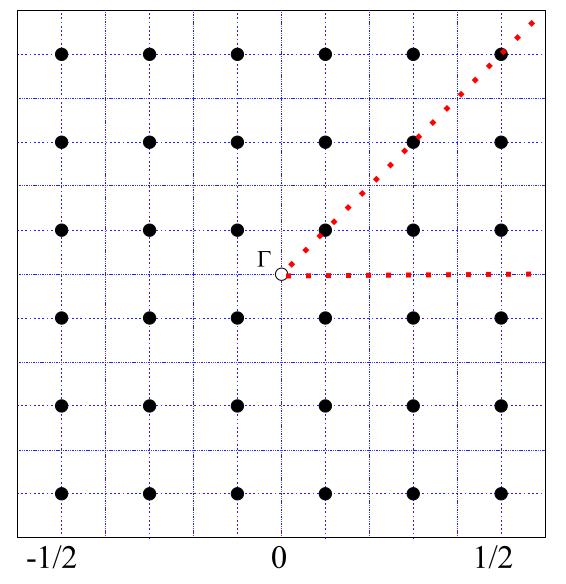
\includegraphics[height=1.5in,width=2.05in,viewport=-200 0 850 800,clip]{Figures/Special-points-MP.png}
\caption{\tiny \textrm{The generation of special $\vec k$-points in \textrm{Monkhorst-Pack} method.}}%
\label{Special-points-MP}
\end{minipage}
\end{figure} 
	\end{itemize}
}

\frame
{
	\frametitle{\textrm{Monkhorst-Pack}布点方案}
	对完全对称化函数$f(\vec k)$,用$A_m(\vec k)$展开
	$$f(\vec k)=\sum_{m=0}^{\infty}f_mA_m(\vec k)$$
	因为$A_m(\vec k)$在\textrm{Brillouin-zone}正交,可得
	$$f_m=\dfrac{V_G}{(2\pi)^3}\int_{\mathrm{BZ}}\mathrm{d}\vec kA_m^{\ast}(\vec k)f(\vec k)$$
	由此可得函数$f(\vec k)$~在\textrm{Brillouin-zone}积分
	$$\int_{\mathrm{BZ}}\mathrm{d}\vec kf(\vec k)=\dfrac{(2\pi)^2}{V_G}f_0$$
	\textcolor{blue}{可见\textrm{Monkhorst-Pack}方案与\textrm{Chadi-Cohen}方案是一致的}
}

\frame
{
	\frametitle{\textrm{Monkhorst-Pack}布点方案}
	考虑晶格点群对称性,%对$\vec k$~点数的求和可以变成不等价点$\vec k_j$~和每个$\vec k_j$~点的等价数的权重$w_j$求和表示\\
	如果$P(q)$是一套$\vec k$~点($\{\vec k_{prs}\}$)中不可约\textrm{Brillouin-zone}的$\vec k_j$~的对称性关联的等价点数,对$f_m$用一套离散的$\vec k_j$~点近似求和可以表示为
	$$\bar f_m=\dfrac1{q^3}\sum_{j=1}^{P(q)}w_j(q)f(\vec k_j)A_m(\vec k_j)$$
%	其中
%	$$w_j^{ab}=\dfrac1q\sum_{r=1}^q\mathrm{e}^{(\mathrm{i}\pi/q)(2r-q-1)(R_j^b-R_j^a)}$$
%	可有
%	\begin{displaymath}
%		W_j^{ab}(q)=\left\{
%		\begin{aligned}
%			&1 \qquad\qquad\mathrm{if}\, |R_j^b-R_j^a|=0,2q,4q,\cdots \\
%			&(-1)^{q+1}\quad \mathrm{if}\, |R_j^b-R_j^a|=q,3q,5q,\cdots \\
%			&0 \qquad\qquad\mathrm{otherwise}
%		\end{aligned}
%		\right.
%	\end{displaymath}
	由此得到$f(\vec k)$~的近似表达$\bar f(\vec k)$表示为
	$$\bar f(\vec k)=\sum_m\bar f_mA_m(\vec k)$$
	对$m$~的求和满足\textcolor{red}{布点约束条件}
	$$|R_j^a|<q/2,\,|R_j^b|<q/2\quad(j=1,2,3)$$
	其中$q$,$R_j^a$,$R_j^b$是整数
}

\frame
{
	\frametitle{\textrm{Monkhorst-Pack}布点的误差}
	\textrm{Monkhorst-Pack}\,布点积分的误差定义
	$$\epsilon_{\mathrm{BZ}}\equiv\int_{\mathrm{BZ}}\mathrm{d}\vec k[f(\vec k)-\bar f(\vec k)]=\sum_{m>1}f_mN_m^{1/2}S_{m1}(q)$$
	这里
	\begin{displaymath}
		S_{m1}(q)=\left\{
		\begin{aligned}
			&(-1)^{(q+1)(R_1+R_2+R_3)/q}\quad \mathrm{if}\; R_1-R_3\; \mathrm{are\, multiples\, of\, q} \\
			&\quad\qquad\qquad 0 \qquad\qquad\qquad \mathrm{otherwise}
		\end{aligned}
		\right.
	\end{displaymath}
	\textcolor{blue}{实际计算中,很多体系的积分与占据数有关,这样只有\textrm{Fermi}面包围的区域对积分有贡献}
	$$\int_{<\mathrm{FS}}\mathrm{d}\vec k f(\vec k)\approx\sum_m\bar f_mI_m(\vec k)$$
	其中
	$$I_m=\int_{<\mathrm{FS}}\mathrm{d}\vec k A_m(\vec k)$$
}

\frame
{
	\frametitle{\textrm{Monkhorst-Pack}布点的误差}
	因此,对\textrm{Fermi}面的积分误差是
	\begin{displaymath}
		\begin{aligned}
			\epsilon_{<\mathrm{FS}}&\equiv\int_{<\mathrm{FS}}\mathrm{d}\vec k[f(\vec k)-\bar f(\vec k)]\\
			&=\sum_m(f_m-\bar f_m)I_m+\sum_{m^{\prime}}f_{m^{\prime}}I_{m^{\prime}}
		\end{aligned}
	\end{displaymath}
	其中对$m^{\prime}$的求和表示求和部分不满足布点约束条件

	\begin{itemize}
		\item \textcolor{red}{当$\vec k_j$~求和遍历\textrm{Brillouin-zone}全部不可约区域,\textrm{Monkhorst-Pack}方法积分是精确和高效的}
		\item \textcolor{blue}{对于立方晶系,$q$~值尽量取为偶数}\\
			目的:~避免选择类似$\Gamma$~点这样的高对称性点,得到更合理的统计平均值
	\end{itemize}
}

\frame
{
	\frametitle{导体的\textrm{Fermi}~面与展宽}
	\begin{itemize}
		\item 由于导体的\textrm{Fermi}~面穿过某些能带,因此被积函数在\textrm{Fermi}~面上是不连续的,积分随$\vec k$~点收敛很慢
		\item 引入含有展宽\textrm{(smearing)}参数$W$的分布函数(如\textrm{Gaussian~}、\textrm{Lorentz~}等函数)可以有效地提升导体在\textrm{Fermi~}面附近的$\vec k$~点收敛性
	\end{itemize}
	计算积分
	$$I=\int_{\mathrm{BZ}}S(E(\vec k)-E_{\mathrm F})f(\vec k)\mathrm{d}\vec k=\int_{-\infty}^{\infty}S(\varepsilon-E_{\mathrm F})f(\varepsilon)\mathrm{d}\varepsilon$$
	这里$$F(\varepsilon)=\int_{\mathrm{BZ}}f(\vec k)\delta(\varepsilon-E(\vec k))\mathrm{d}\vec k$$
	$E(\vec k)$是能带的色散关系,$E_{\mathrm F}$是\textrm{Fermi~}能级,$f(\vec k)$~是被积函数
	\begin{displaymath}
		S(x)=1-\theta(x)=\left\{
		\begin{aligned}
			1\quad x\leqslant0\\
			0\quad x>0
		\end{aligned}\right.
	\end{displaymath}
}

\frame
{
	\frametitle{导体的\textrm{Fermi}~面与展宽}
	当\textrm{step~}函数$S(x)$用\textrm{Fermi-Dirac}分布函数代替,可以很好地提升$\vec k$~点收敛性,但因此引入了误差
	\begin{figure}[h!]
	\centering
	\vspace*{-0.2in}
	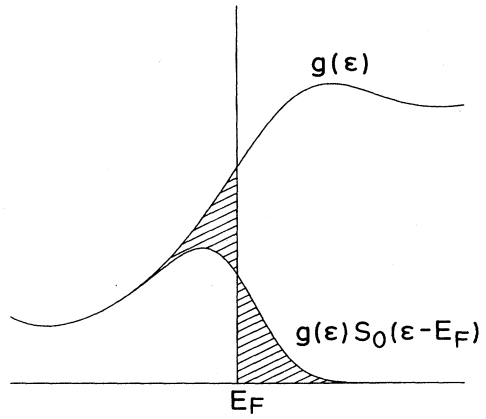
\includegraphics[height=1.1in,width=1.25in,viewport=0 0 530 500,clip]{Figures/MP_distribution.png}
	\caption{\textrm{A schematic density of states $g(\varepsilon)$ and function multiplied by a smooth distribution function.}}%
	\label{MP_distribution}
	%\hspace*{-10pt}
	\end{figure} 
	\textrm{Methfessel-Paxton~}提出用更复杂的多项式函数$S_N$\upcite{PRB40-3616_1989},引入变量$x=(\varepsilon-E_{\mathrm F})/W$,为了用函数$S_N(x)$逼近\textrm{Step~}函数$S(x)$,%,并要求$S_N$是平滑函数
	先用\textrm{Hermite~}多项式展开$\delta(x)$
	\vspace*{-8pt}
	\begin{displaymath}
		\delta(x)=\sum_{n=0}^{\infty}A_nH_{2n}(x)\mathrm{e}^{-x^2}
	\end{displaymath}
}

\frame
{
	\frametitle{导体的\textrm{Fermi}~面与展宽}
	利用\textrm{Hermite~}多项式的正交性和\textrm{Gaussian~}权重
	\begin{displaymath}
		\int_{-\infty}^{\infty}H_n(x)H_m(x)\mathrm{e}^{-x^2}\mathrm{d}x=n!2^n\sqrt{\pi}\delta
	\end{displaymath}
	可得系数$A_n$
	\begin{displaymath}
		A_n=\frac{H_{2n}(0)}{(2n)!4^n\sqrt{\pi}}=\frac{(-1)^n}{n!4^n\sqrt{\pi}}
	\end{displaymath}
	因此有$\delta$函数的逼近函数
	\begin{displaymath}
		D_N(x)=\sum_{n=0}^NA_nH_{2n}(x)\mathrm{e}^{-x^2}
	\end{displaymath}
	由此得到\textrm{Step}~函数的逼近函数
	\begin{displaymath}
		S_N(x)=1-\int_{-\infty}^xD_N(t)\mathrm{d}t
	\end{displaymath}
}

\frame
{
	\frametitle{逼近函数}
	利用等式$$\frac{\mathrm d}{{\mathrm d}x}[H_n(x)\mathrm{e}^{-x^2}]=-H_{n+1}(x){\mathrm e}^{-x^2}$$
	\begin{figure}[h!]
		\begin{minipage}[t]{0.55\linewidth}
			可得\textrm{Methfessel-Paxton~}积分
		\begin{displaymath}
			\begin{aligned}
				S_0(x)&=\frac12\left[1-\mathrm{erf}(x)\right]\\
				S_N(x)&=S_0(x)+\sum_{n=1}^NA_nH_{2n-1}(x)\mathrm{e}^{-x^2}
			\end{aligned}
		\end{displaymath}
		\textcolor{blue}{$S_0$对应于\textrm{Gaussian}分布函数}(类似\textrm{Fermi-Dirac}分布函数)
		\end{minipage}
		\hfill
		\begin{minipage}[t]{0.40\linewidth}
		\centering
		\vspace*{-0.8in}
%		\hspace*{0.5in}
		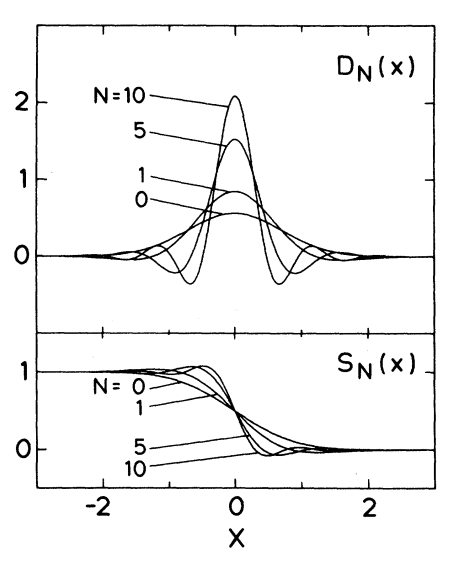
\includegraphics[height=2.0in,width=1.25in,viewport=0 0 530 800,clip]{Figures/MP_SN_DN.png}
		\caption{\fontsize{4.1pt}{3.9pt}\selectfont{\textrm{Sucessive approximants to the $\delta$ function, $D_N$ and to the step function $S_N$.}}}%
		\label{MP_SN_DN}
		%\hspace*{-10pt}
		\end{minipage}
	\end{figure} 
	\textrm{Methfessel-Paxton~}提出用更复杂的多项式函数$S_N$,引入变量$x=(\varepsilon-E_{\mathrm F})/W$,为了用函数$S_N(x)$逼近\textrm{Step~}函数$S(x)$%,并要求$S_N$是平滑函数
}

\frame
{
	\frametitle{逼近函数的属性}
	如果有不多于\textrm{2N+1~}项的多项式$P(x)$
	\begin{displaymath}
		\int_{-\infty}^{\infty}D_N(x)P(x)\mathrm{d}x=\int_{-\infty}^{\infty}\delta(x)P(x)\mathrm{d}x=P(0)
	\end{displaymath}
	因此$P(x)$可以用\textrm{Hermite}多项式展开
\begin{itemize}
	\item \begin{displaymath}
			0=\int_{-\infty}^{\infty}\left[D_N(x)-\delta(x)\right]P(x)\mathrm{d}x
	\end{displaymath}
	\item \begin{displaymath}
			0=\int_{-\infty}^{\infty}\left[S_N(x)-S(x)\right]P(x)\frac{{\mathrm d}}{\mathrm dx}\mathrm{d}x
	\end{displaymath}
\end{itemize}
可见$S_N(x)$是对\textrm{Step}函数$S(x)$的很好逼近,当$F(x)$可用不多于\textrm{2N+1~}项多项式表示,则积分误差
$$\int\left[S_N(x)-S(x)\right]F(x)\mathrm{d}x\sim\textcolor{red}{\mathrm{e}^{-x^2}}$$
}

\subsection{四面体布点与积分方法}
\frame
{
	\frametitle{四面体布点方案}
	四面体方法是更普适的一般方法,除了可用于绝缘体、半导体、金属的期望值计算,还可以计算体系的谱函数,即体系的动态响应性质。\upcite{PRB49-16223_1994}

	四面体积分基本思想
	\begin{enumerate}
		\item 为了计算$\vec k$~空间积分,四面体方法先将第一\textrm{Brillouin-zone}分割成若干等体积的小四面体
		\item 计算每个四面体对积分权重的贡献
		\item 对所有四面体贡献权重求和
	\end{enumerate}
	\begin{displaymath}
		\langle X_n\rangle=\dfrac1{V_G}\int_{V_G}\mathrm{d}\vec kX_n(\vec k)f(\vec k)=\dfrac1{V_G}\sum_{j=1}^{N_{\mathrm{Tet}}}\int_{V_T}\mathrm{d}\vec kX_n(\vec k)f(\varepsilon_n^{\vec k})
	\end{displaymath}
	相应地每个\textrm{Brillouin-zone}不可约$\vec k$点积分权重$w_{nj}$
	\begin{displaymath}
		w_{nj}=\dfrac1{V_G}\int_{V_G}\mathrm{d}\vec kw_j(\vec k)f(\varepsilon_n^{\vec k})
	\end{displaymath}
}

\frame
{
	\frametitle{四面体布点方案}
	\textcolor{blue}{对于完全占据的四面体区域},$X_n(\vec k)$在每个四面体上的积分为
	\begin{displaymath}
		\dfrac1{V_G}\int_{V_T}\mathrm{d}\vec k X_n(\vec k)=\dfrac{V_T}{V_G}\sum_{j=1}^4\textcolor{blue}{\dfrac14}X_n(\vec k_j)
	\end{displaymath}
	这里积分权重$w_j=\frac14$来自线性插值积分
	$$w_j=\int_{V_T}\mathrm{d}\vec k\quad j=1,2,3$$
	而$w_4=1-\sum\limits_{j=1}^3w_j$

	\textcolor{red}{当\textrm{Fermi}面部分穿越四面体的时候,只有四面体中能级$\varepsilon<\varepsilon_{\mathrm{F}}$的体积对积分有贡献},因此
	\begin{displaymath}
		\dfrac1{V_G}\int_{V_T}\mathrm{d}\vec k X_n(\vec k)=\dfrac{V_T}{V_G}\sum_{j=1}^4X_n(\vec k_j)\textcolor{red}{w_j}
	\end{displaymath}
}

\frame
{
	\frametitle{四面体布点方案}
\begin{figure}[h!]
\begin{minipage}[t]{0.45\linewidth}
\centering
\includegraphics[height=1.25in,width=1.50in,viewport=15 15 250 190,clip]{Figures/Tetrahedron.eps}
\caption{\tiny Arrangement of the secant plane of constant energy in the method of tetrahedrons when $\varepsilon_0\leqslant\varepsilon_F\leqslant\varepsilon_1$.}%(与文献\cite{EPJB33-47_2003}图1对比)
\label{Fig:Tetrahedron}
\end{minipage}
\hfill
\begin{minipage}[t]{0.50\linewidth}
	\vspace*{-100pt}
	在每个四面体内,等能面$\varepsilon$的线性插值表示
		\begin{displaymath}
			\begin{aligned}
				\vec k_{10}(\varepsilon)=&\vec k_{10}\frac{\varepsilon-\varepsilon_0}{\varepsilon_1-\varepsilon_0}\\
				\vec k_{20}(\varepsilon)=&\vec k_{20}\frac{\varepsilon-\varepsilon_0}{\varepsilon_2-\varepsilon_0}\\
				\vec k_{30}(\varepsilon)=&\vec k_{30}\frac{\varepsilon-\varepsilon_0}{\varepsilon_3-\varepsilon_0}\\
			\vec k_0(\varepsilon)=&\vec k_0+a_1\vec k_{10}(\varepsilon)+a_2\vec k_{20}(\varepsilon)\\
			+&a_3\vec k_{30}(\varepsilon)
			\end{aligned}
		\end{displaymath}
		\hspace*{-15pt}引入矢量$g_{i0}$,满足$\vec g_{i0}\vec k_{j0}=\delta_{ij}$
\end{minipage}
\end{figure}
%\vspace*{-5pt}
		$$\varepsilon(\vec k)=\varepsilon_0+\sum_i^3(\varepsilon_i-\varepsilon_0)\vec g_{i0}(\vec k-\vec k_0)=\varepsilon_0+(\varepsilon-\varepsilon_0)(a_1+a_2+a_3)$$
%		根据条件$\varepsilon=\varepsilon_i(i=1,2,3)$确定系数
}

\frame
{
	\frametitle{四面体积分权重的确定}
\begin{figure}[h!]
\centering
\subfigure[\textrm{\small Arrangement of the different secant planes of constant energy in the method of tetrahedrons}]{
\label{Fig:Tetra-equal-ene}
\vspace*{-0.25in}
	\includegraphics[height=1.55in,width=2.03in,viewport=40 125 530 465,clip]{Figures/Tetra-equal-ene.eps}}
	\hfill
\subfigure[\textrm{\small Two-dimensional schematic illustration of the function $w_j(\vec k)$.}]{
\label{Fig:dime_Tetra}
\vspace*{-0.25in}
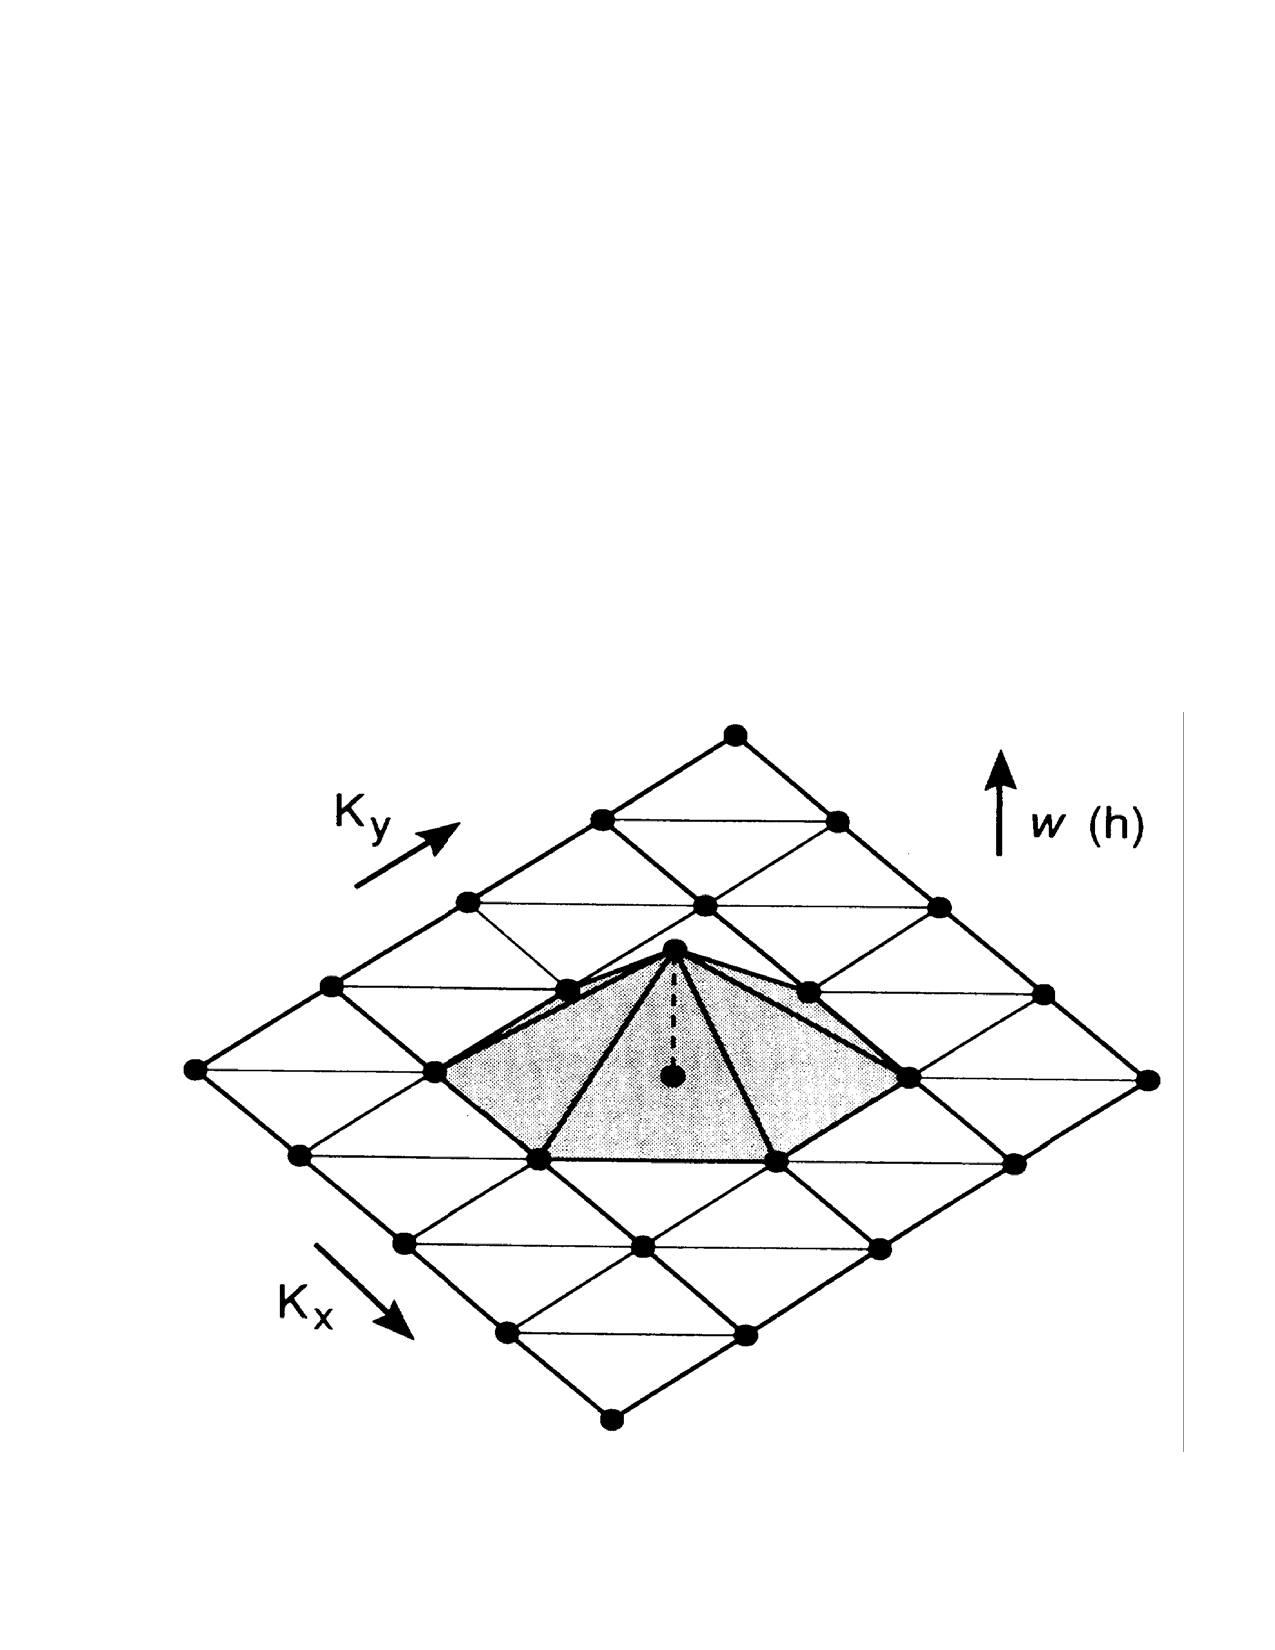
\includegraphics[height=1.75in,width=1.75in,viewport=0 30 565 505,clip]{Figures/dimen_Tetra.pdf}}
\end{figure}
根据能量范围的不同,可以推导出不能能量区域内的积分权重的表达式,详见文献\cite{PRB49-16233_1994}的附录
}

\frame
{
	\frametitle{四面体的生成}
%类似地,可以有四面体方法态数目(\textrm{number of states})、态密度(\textrm{Density of States, DOS})$D_T(\varepsilon_i)$的贡献表达式,具体可参见文献\cite{PRB49-16233_1994}。
	为了减少统计四面体的数目,可以先找出第一\textrm{Brillouin-zone}的不可约部分。但这一策略有副作用,\textcolor{red}{由于不可约部分的不规则性,其中的四面体划分几乎不可避免地要人工干预,不利于编程求解}\\\textrm{Bl\"ochl}提出一个解决方法:\\
\begin{enumerate}
	\item 利用\textrm{Monkhorst-Pack}方案\upcite{PRB13-5188_1976}首先在第一\textrm{Brillouin-zone}内生成等体积的平行六面体网格。
	\item 依次给每个点编号:
\begin{displaymath}
	\boxed{N=1+\dfrac{i-i_0}2+(n_1+1)\left[\dfrac{j-j_0}2+(n_2+1)\dfrac{k-k_0}2\right]}
\end{displaymath}
其中$i,j,k$分别是该$\vec k$~点沿倒格矢$\mathbf{b}_i(i=1,2,3)$的序数的二倍,$i_0,j_0,k_0$是\textrm{Monkhorst-Pack}方法中点的偏移量,有偏移则为1,否则为0。
\end{enumerate}
}

\frame
{
	\frametitle{四面体的生成}
\begin{enumerate}
	\setcounter{enumi}{2}
	\item 编号之后建立标识数组,其位置与该位置储存的元素值相同,例如,第一个位置存储“$1$”,第二个位置存储“$2$”,依次类推
	\item 然后从第一个位置开始,利用对称群的操作矩阵对每个点坐标作用,并与数组中其他点的坐标进行比较,如果彼此相同且后者的编号大于前者,即将后者的元素值改为前者\\\textcolor{blue}{对全部数组操作完毕,可以挑出所有不可约$\vec k$~点:\\只有当$\vec k_i$~为不可约$\vec k$~点时,其编号才与其存储位置相同}。
	\item 为了计算方便,可以对所有这些不可约$\vec k$~点按存储位置的顺序重新编号,即从“$1$”到“$\vec k_{\mathrm{irr}}(\max)$”。数组中的各个元素也相应的改为新的编号。这样整个第一\textrm{Brillouin-zone}中的点都可用不可约点标记。
\end{enumerate}
}

\frame
{
	\frametitle{四面体的生成}
下一步讨论四面体的自动划分过程

以下八组坐标代表的点构成平行六面体:
\begin{displaymath}
	\begin{aligned}
		&(l,m,n)\rightarrow 1,&(l+1,m,n)\rightarrow 2\\
		&(l,m+1,n)\rightarrow 3,&(l+1,m+1,n)\rightarrow 4\\
		&(l,m,n+1)\rightarrow 5,&(l+1,m,n+1)\rightarrow 6\\
		&(l,m+1,n+1)\rightarrow 7,&(l+1,m+1,n+1)\rightarrow 8
	\end{aligned}
\end{displaymath}
为了尽量减小插值引起的误差,可以取此平行六面体中最短的体对角线作为等体积的六个四面体的公共对角线,设为$3-6$,则可以采用下面6组途径确定这六个四面体的各个顶点:
\begin{displaymath}
	\begin{aligned}
		1\rightarrow2\rightarrow3\rightarrow6\quad&1\rightarrow3\rightarrow5\rightarrow6\quad&2\rightarrow3\rightarrow4\rightarrow6\\
		3\rightarrow5\rightarrow6\rightarrow7\quad&3\rightarrow4\rightarrow6\rightarrow8\quad&3\rightarrow6\rightarrow7\rightarrow8
	\end{aligned}
\end{displaymath}
}

\frame
{
	\frametitle{四面体的生成}
\begin{figure}[h!]
\centering
\vspace*{-0.28in}
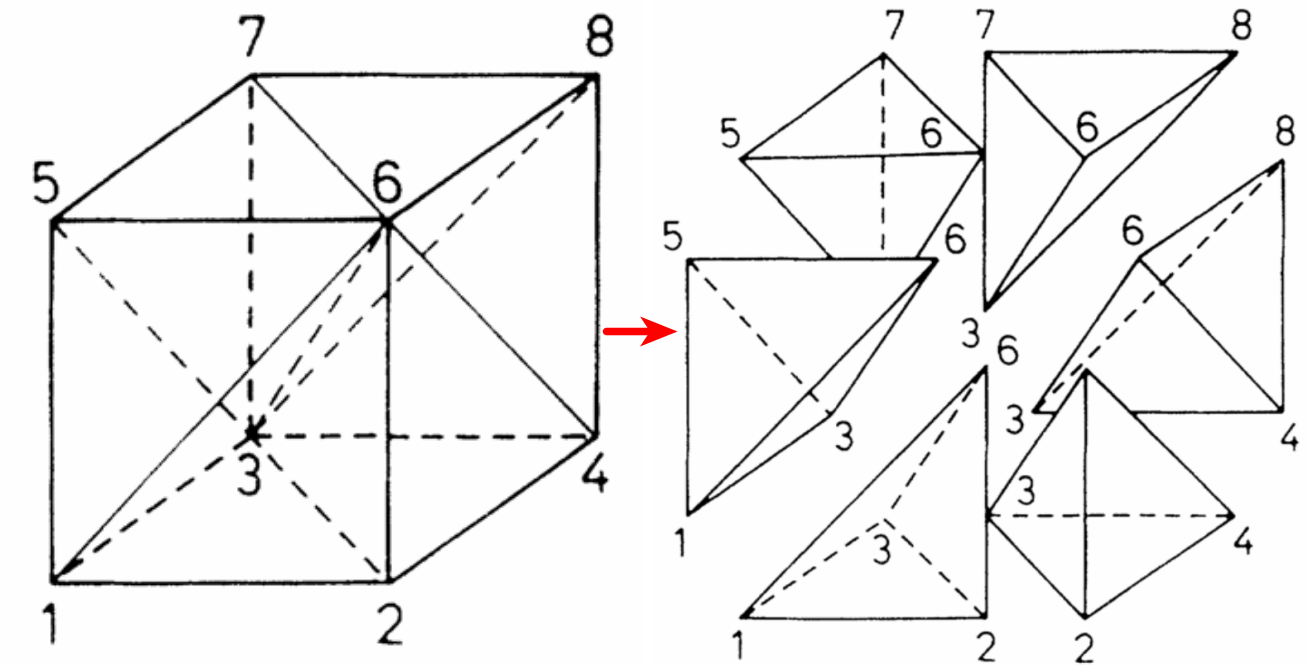
\includegraphics[height=1.25in,width=3.00in,viewport=0 0 1350 705,clip]{Figures/submesh_Tetra.png}
\caption{\tiny Breakup of a submesh cell into six tetrahedra.}%(与文献\cite{EPJB33-47_2003}图1对比)
\label{Fig:Submesh_Tetra}
\end{figure}
对每个平行六面体重复上述过程,将第一\textrm{Brillouin-zone}划分为体积相等的若干四面体,每个四面体的顶点可用标识数组中的不可约点标记。将这四个顶点的标号按升序排列,可以方便地确定等价四面体(简并度)\\
这个过程保证了\textcolor{red}{只用不可约点上的信息进行整个第一\textrm{Brillouin}区的积分,无须考虑如何划定其不可约部分}\\
%上述过程可以避免Kleinman所说的计算误差,而且整个过程可以通过程序自动实现而无须人工干预。
上述过程可以避免计算误差,而且整个过程可以通过程序自动实现而无须人工干预
}

\frame
{
	\frametitle{四面体积分的误差}
	四面体积分的误差有两个来源
	\begin{itemize}
		\item 四面体内的线性插值引入的误差
		\item 四面体内等能面线性插值逼近真实\textrm{Fermi~}面引入的误差
	\end{itemize}
\begin{figure}[h!]
\centering
\vspace*{-0.28in}
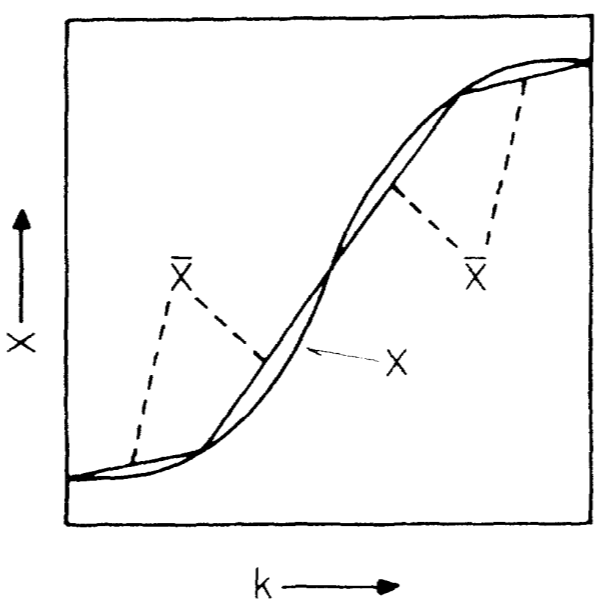
\includegraphics[height=1.25in,width=1.25in,viewport=0 0 650 650,clip]{Figures/Tetra_error.png}
\caption{\tiny Schematic representation of the interpolation error due to line interpolation.}%(与文献\cite{EPJB33-47_2003}图1对比)
\label{Fig:Tetra_error}
\end{figure}
\textcolor{blue}{对半导体和绝缘体,由于价带被完全填充,用\textrm{Monkhorst-Pack~}布点产生四面体积分方案,可以保证积分误差完全抵消}
}

\frame
{
	\frametitle{四面体积分的误差估计}
		对导体材料,每个四面体内的线性插值积分误差
	\begin{displaymath}
		\delta\langle X\rangle_T=\int_T\mathrm{d}^3k\left[ X(\vec k)-\bar X(\vec k) \right]
	\end{displaymath}
为估计积分误差,假设有被积函数
$$X(\vec k)=a+\sum_ib_ik_i+\frac12\sum_{ij}k_ic_{ij}k_j$$
四面体的一个顶点置于原点,其余三个点位于$\vec t_i=(t_{1i},t_{2i},t_{3i})$,其中$i=1,2,3$
\begin{figure}[h!]
\centering
\vspace*{-0.3in}
\includegraphics[height=1.65in,width=1.70in,viewport=15 15 500 550,clip]{Figures/Brillouin-Tetra.eps}
%\caption{\tiny .}%(与文献\cite{EPJB33-47_2003}图1对比)
\label{Fig:Brillouin-Tetrahedron}
\end{figure}
}

\frame
{
	\frametitle{四面体积分的误差估计}
变换坐标系$s_i$
$$k_i=\sum_jt_{ij}s_j$$
因此被积函数变换为
$$X(\vec s)=\bar a+\sum_i\bar b_is_i+\frac12\sum_{ij}s_i\bar c_{ij}s_j$$
这里系数$\bar a=a$,$\bar b_i=\sum\limits_jb_jt_{ji}$,$\bar c_{ij}=\sum\limits_{kl}t_{kl}c_{kl}t_{lj}$\\
并且$s_i>0\;i=1,2,3$,$\sum\limits_{i=1}^3s_i\leqslant1$

因此可有被积函数的线性插值为
$$\bar X(\vec s)=\bar a+\sum_i(\bar b_i+\frac12\bar c_{ii})s_i$$
}

\frame
{
	\frametitle{四面体积分的误差估计}
	因此积分误差可以解析表示为
	\begin{displaymath}
		\begin{aligned}
			\delta\langle X\rangle_T=&\mathrm{det}|t_{ij}|\int_T\mathrm{d}^3s\frac12\left[ \sum_{ij}s_i\bar c_{ij}s_j-\sum_i\bar c_{ii}s_i \right]\\
			=&\frac16\mathrm{det}|t_{ij}|\frac1{40}\left[ \sum_{i\neq j}\bar c_{ij}-3\sum_i\bar c_{ii} \right]
		\end{aligned}
	\end{displaymath}
	将$c_{ij}$用被积函数的二阶导数表示,$\frac16\mathrm{det}|t_{ij}|$是四面体体积$V_T$,因此可有
	\begin{displaymath}
		\delta\langle X\rangle_T=V_T\sum_{ij}\left\langle\frac{\partial^2X}{\partial k_i\partial k_j}\right\rangle_TC_{ii}\Delta^2
	\end{displaymath}
	这里$\Delta=\sqrt[3]{\mathrm{det}|t|}$
	$$C_{ij}=\frac1{40\Delta^2}\left[ \sum_{l\neq m}t_{il}t_{jm}-3\sum_lt_{ij}t_{jl} \right]$$
}

\frame
{
	\frametitle{四面体积分的误差估计}
	对全部占据四面体误差$\delta\langle X\rangle_T$求和,得到插值误差
	\begin{displaymath}
		\delta\langle X\rangle=\left\langle\sum_{ij}\frac{\partial^2X}{\partial k_i\partial k_j}C_{ii}\right\rangle\Delta^2
	\end{displaymath}
	因此\textcolor{red}{四面体积分误差随$\Delta^2$收敛}

	\textcolor{blue}{根据\textrm{Green's~}积分公式,可将体相积分变成\textrm{Fermi~}面的表面积分}
	\begin{displaymath}
		\begin{aligned}
			\delta\langle X\rangle=&\frac1{V_G}\sum_{ij}\langle C_{ij}\rangle\int_{V_G}\mathrm{d}^3k\frac{\partial^2X}{\partial k_i\partial k_j}\Delta^2\\
			=&\frac1{V_G}\sum_{ij}\langle C_{ij}\rangle\oint_{\varepsilon=\varepsilon_{\mathrm F}}\mathrm{d}^2A_i\frac{\partial X}{\partial k_j}\Delta^2
		\end{aligned}
	\end{displaymath}
因此可有
	\begin{displaymath}
			\delta\langle X\rangle=\frac1{V_G}\sum_{ij}\oint_{\varepsilon=\varepsilon_{\mathrm F}}\mathrm{d}^2A_iC_{ij}\frac{\partial X}{\partial k_j}\Delta^2
	\end{displaymath}
}

\frame
{
	\frametitle{四面体积分的误差}
\vspace*{-10pt}
	将如下关系
	\begin{displaymath}
		\begin{aligned}
		&\int\mathrm{d}^2A_i=\int\mathrm{d}^2|A|\frac1{\nabla_k\varepsilon}\frac{\partial\varepsilon}{\partial k_i}\\
		&\sum_i\frac{\partial\varepsilon}{\partial k_i}t_{ij}=\varepsilon_{j+1}-\varepsilon_1\\
		&\sum_i\frac{\partial X}{\partial k_i}t_{ij}=X_{j+1}-X_1 
		\end{aligned}
	\end{displaymath}
这里$\varepsilon_i$和$X_i$是四面体顶点的能量和被积函数值,
\vspace*{-5pt}
\begin{displaymath}
	\begin{aligned}
		\delta\langle X\rangle=&\sum_TD_T(\varepsilon_{\mathrm F})\frac1{40}\left[\sum_{i\neq j}(X_{i+1}-X_1)(\varepsilon_{j+1}-\varepsilon_1)\right.\\
			&-3\left.\sum_i(X_{i+1}-X_1)(\varepsilon_{j+1}-\varepsilon_1)\right]\\
			=&\sum_TD_T(\varepsilon_{\mathrm F})\frac1{40}\sum_{i=1}^4X_i\sum_{j=1}^4(\varepsilon_j-\varepsilon_i) 
	\end{aligned}
\end{displaymath}
}

\frame
{
	\frametitle{四面体积分权重校正}
	\textcolor{red}{四面体积分权重校正为}
\begin{displaymath}
	\mathrm{d}w_i=\frac{\delta\langle X\rangle}{\delta X_i}=\sum_T\frac1{40}D_T(\varepsilon_{\mathrm F})\sum_{j=1}^4(\varepsilon_j-\varepsilon_i) 
\end{displaymath}

类似地,考虑等能面线性插值对\textrm{Fermi~}面逼近引起的误差,可得\\\textcolor{blue}{每个四面体的电子数校正}
\begin{displaymath}
	\delta N_{\mathrm{el},T}=\frac{A_T}{V_G}\sum_{ij}\frac{\partial^2k_{\mathrm F}}{\partial k_i\partial k_j}C_{ij}\Delta^2
\end{displaymath}
这里$A_T$是三角形面积
	$$C_{ij}=\frac1{24\Delta^2}\left[ \sum_{l\neq m}t_{il}t_{jm}-2\sum_lt_{ij}t_{jl} \right]$$
	其中$t_{ij}$是与四面体类似的三角形顶点适量\\
	\textcolor{red}{对均匀电子,四面体积分误差随$\Delta^3$收敛}
}

\frame
{
	\frametitle{四面体积分的积分权重与展宽}
	\textcolor{red}{四面体$W=\dfrac{\mathrm{d}w_i}{\mathrm{d}\varepsilon}$对能量导数对应于“展宽”}
\begin{figure}[h!]
\centering
\vspace*{-0.28in}
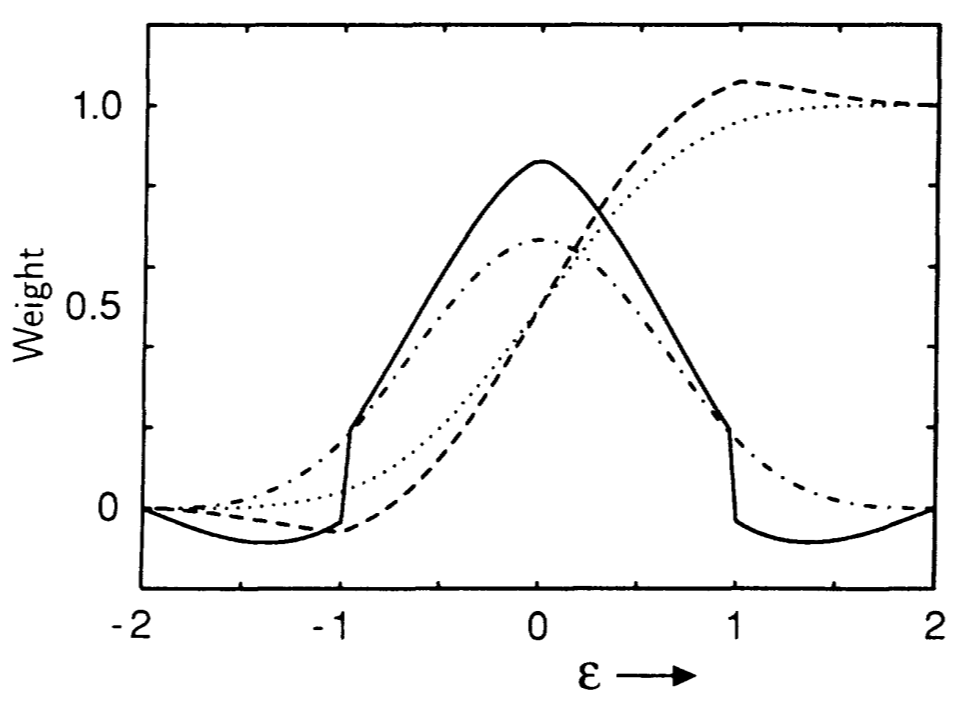
\includegraphics[height=1.4in,width=1.55in,viewport=0 0 1000 800,clip]{Figures/Tetra_smearing.png}
%\caption{\tiny .}%(与文献\cite{EPJB33-47_2003}图1对比)
\label{Fig:Tetrahedron-smearing}
\end{figure}
\begin{itemize}
\vspace*{-0.1in}
	\item \textcolor{blue}{四面体方法展宽参数可随能带分布和形状\\
	传统展宽方法的展宽系数对所有能带都相同}
	\item \textcolor{red}{四面体方法不推荐引入展宽参数}\\
		\begin{enumerate}
			\item 展宽计算的总能不满足变分原理,\textrm{Hellmann-Feynman}定理不再满足,\textcolor{red}{不能正确计算导体的受力}
			\item 四面体能保证态密度计算在\textrm{van Hove}奇点附近出现振荡,引入展宽会破坏这一特征
		\end{enumerate}
\end{itemize}
}

\frame
{
\frametitle{四面体布点积分方案}
\begin{figure}
\centering
\begin{minipage}[b]{0.45\linewidth}
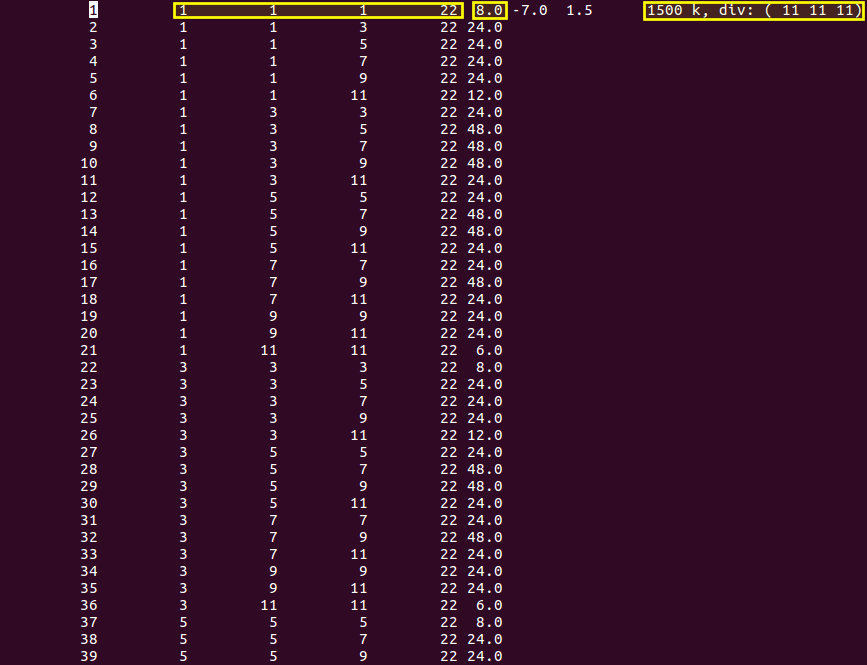
\includegraphics[height=0.65\textheight,width=1.07\textwidth,viewport=70 0 900 700,clip]{Figures/WIEN2k_CaB6-klist.png}
\caption{\tiny{\textrm{case.klist}}}
\end{minipage}
\begin{minipage}[b]{0.45\linewidth}
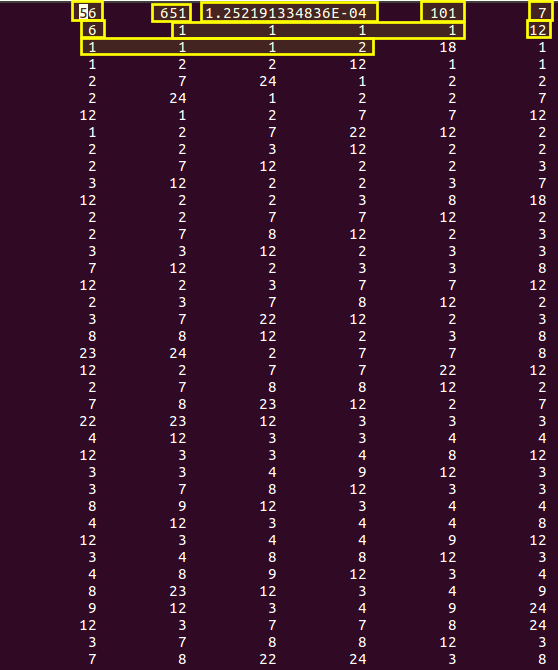
\includegraphics[height=0.65\textheight,width=1.0\textwidth,viewport=0 0 670 700,clip]{Figures/WIEN2k_CaB6-kgen.png}
\caption{\tiny\textrm{case.kgen}}
\end{minipage}
\end{figure}
}

\frame
{
	\frametitle{各种$\vec k$~空间积分方法的比较}
\vskip -7pt
\begin{footnotesize}
\arrayrulewidth=0.4pt
\doublerulesep=0.4pt
\begin{table}[!h]
\tabcolsep 0pt \vspace*{-12pt}
%\begin{minipage}{\textwidth}
\label{tab:magno-1}
\centering
\def\temptablewidth{1.01\textwidth}
{\rule{\temptablewidth}{0.8pt}}
\begin{tabular*} {\temptablewidth}{|c@{\extracolsep{\fill}}|c|c|c|c|}
	\multirow{3}{*}{\textcolor{red}{积分方案}}	&\multicolumn{4}{c|}{\textcolor{blue}{布点方案}:~\textrm{Monkhorst-Pack}~方法} \\\cline{2-5}
	&\multirow{2}{*}{\textrm{Fermi-Dirac}~方法} &\multicolumn{2}{c|}{\textrm{Methfessel-Paxton}~方法} &\multirow{2}{*}{\textrm{Tetrahedron}~方法}\\\cline{3-4}
& &\textrm{Gaussian~} &$N>0$ & \\ \hline
半导体、&\multirow{2}{*}{\textcolor{blue}{$\texttimes$}} &$\delta\leqslant0.05$ &\multirow{2}{*}{\textcolor{red}{$\texttimes$}} &\textcolor{blue}{\textrm{DOS \& total-Energy}}\\
绝缘体 & &\textcolor{blue}{$\checkmark$} & &\textcolor{red}{$\checkmark$} \\\hline
导体、 & \multirow{2}{*}{\textcolor{blue}{$\checkmark$}} & \multicolumn{2}{c|}{\textcolor{blue}{\textrm{Phonon \& relaxation}}} &\textcolor{blue}{\textrm{DOS \& total-Energy}} \\
金属 & &\multicolumn{2}{c|}{\textcolor{red}{$\checkmark$}}  &\textcolor{red}{$\checkmark$} \\\hline
\multirow{2}{*}{\textrm{supercell}} &\multirow{2}{*}{\textcolor{blue}{$\checkmark$}} &\multicolumn{2}{c|}{\multirow{2}{*}{\textcolor{red}{$\checkmark$}}} &\multirow{2}{*}{\textcolor{red}{$\texttimes$}}\\
& &\multicolumn{2}{c|}{} &\\
\end{tabular*}
{\rule{\temptablewidth}{1pt}}\\
%\end{center}1
%\end{minipage}
\end{table}
\end{footnotesize}
}
%\frame
%{
%\begin{figure}[h!]
%\centering
%\vspace*{-0.25in}
%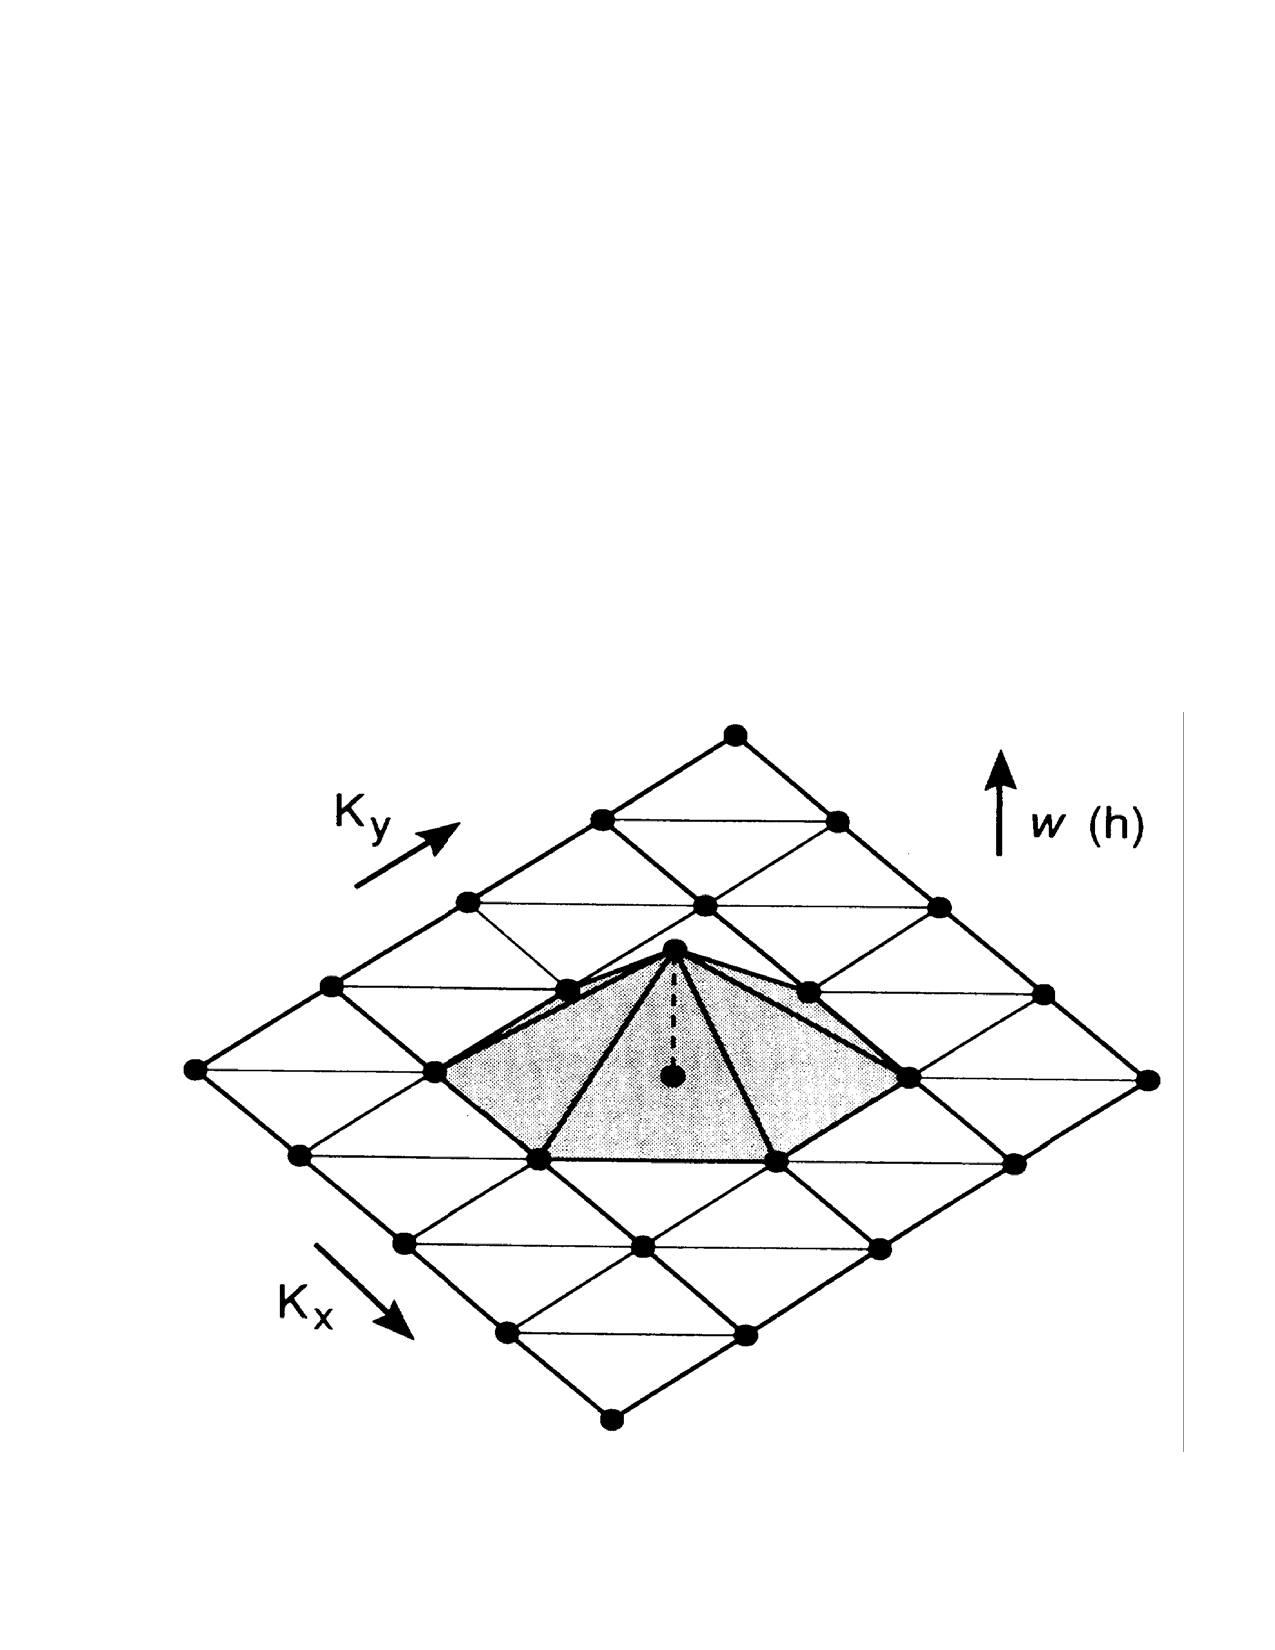
\includegraphics[height=2.75in,width=3.05in,viewport=0 30 565 505,clip]{Figures/dimen_Tetra.pdf}
%\caption{\tiny Two-dimensional schematic illustration of the function $w_j(\vec k)$.}%(与文献\cite{EPJB33-47_2003}图1对比)
%\label{Fig:dime_Tetra-2}
%\end{figure}
%}

%------------------------------------------------------------------------Reference----------------------------------------------------------------------------------------------
		\frame[allowframebreaks]
{
\begin{thebibliography}{99}
\frametitle{主要参考文献}
{\tiny
	\bibitem{PRB7-5212_1973}\textrm{A. Baldereschi \textit{Phys. Rev.} B, \textbf{7} (1973), 5212}
	\bibitem{PRB8-5747_1973}\textrm{D. J. Chadi and M. L. Cohen \textit{Phys. Rev.} B, \textbf{8} (1973), 5747}
	\bibitem{PRB13-5188_1976}\textrm{H. J. Monkhorst and J. D. Pack \textit{Phys. Rev.} B, \textbf{13} (1976), 5188}
	\bibitem{PRB40-3616_1989}\textrm{M. Methfessel and A. T. Paxton \textit{Phys. Rev.} B, \textbf{40} (1989), 3616}
	\bibitem{PRB49-16233_1994}\textrm{P. E. Bl\"ochl, O. Jepsen and O. K. Andersen. \textit{Phys. Rev.} B, \textbf{49} (1994), 16233}
}
\end{thebibliography}
\nocite*{}
}
%-----------------------------------------------------------------------------------------------------------------------------------------------------------------------%

\section{附录:~四面体积分方案的各类权重公式}
\frame
{
	\frametitle{四面体积分中\textrm{Fermi}面的确定}
	已知每个四面体对积分态密度(态数目)$n_T(\varepsilon)$的贡献\upcite{PRB49-16233_1994}
	\begin{itemize}
	\item $\varepsilon<\varepsilon_1$
%		\begin{displaymath}
		\:	$n_T(\varepsilon)=0$
%		\end{displaymath}
	\item $\varepsilon_1<\varepsilon<\varepsilon_2$
%		\begin{displaymath}
		\:	$n_T(\varepsilon)=\dfrac{V_T}{V_G}\dfrac{(\varepsilon-\varepsilon_1)^3}{\varepsilon_{21}\varepsilon_{31}\varepsilon_{41}}$
%		\end{displaymath}
	\item $\varepsilon_2<\varepsilon<\varepsilon_3$
		\begin{displaymath}
			\hspace*{-35pt}	n_T(\varepsilon)=\dfrac{V_T}{V_G}\dfrac1{\varepsilon_{31}\varepsilon_{41}}\left[\varepsilon_{21}^2+3\varepsilon_{21}(\varepsilon-\varepsilon_2)+3(\varepsilon-\varepsilon_2)^2-\dfrac{\varepsilon_{31}+\varepsilon_{42}}{\varepsilon_{32}\varepsilon_{42}}(\varepsilon-\varepsilon_2)^3\right]
		\end{displaymath}
	\item $\varepsilon_3<\varepsilon<\varepsilon_4$
%		\begin{displaymath}
		\:	$n_T(\varepsilon)=\dfrac{V_T}{V_G}\left[1-\dfrac{(\varepsilon_4-\varepsilon)^3}{\varepsilon_{41}\varepsilon_{42}\varepsilon_{43}}\right]$
%		\end{displaymath}
	\item $\varepsilon>\varepsilon_4$
%		\begin{displaymath}
		\:	$n_T(\varepsilon)=\frac{V_T}{V_G}$
%		\end{displaymath}
	\end{itemize}
	利用等能面的插值,由约束条件确定\textrm{Fermi}能级$\varepsilon_{\mathrm F}$
	$$\int_{\varepsilon_0}^{\varepsilon_{\mathrm F}}\sum_{T=1}^{N_{Tet}}n_T(\varepsilon)\mathrm{d}\varepsilon=N_e$$
}

\frame
{
	\frametitle{四面体积分权重的确定}
	不能能量区域内的积分权重的表达式\upcite{PRB49-16233_1994}
	\begin{itemize}
	\item $\varepsilon_F<\varepsilon_1$
		\begin{displaymath}
			\omega_1=\omega_2=\omega_3=\omega_4=0
		\end{displaymath}
	\item $\varepsilon_1<\varepsilon_F<\varepsilon_2$
		\begin{displaymath}
			\begin{aligned}
				\omega_1=&C\bigg[4-(\varepsilon_F-\varepsilon_1)\bigg(\dfrac1{\varepsilon_{21}}+\dfrac1{\varepsilon_{31}}+\dfrac1{\varepsilon_{41}}\bigg)\bigg]\\
				\omega_2=&C\dfrac{\varepsilon_F-\varepsilon_1}{\varepsilon_{21}}\\
				\omega_3=&C\dfrac{\varepsilon_F-\varepsilon_1}{\varepsilon_{31}}\\
				\omega_4=&C\dfrac{\varepsilon_F-\varepsilon_1}{\varepsilon_{41}}
			\end{aligned}
		\end{displaymath}
		这里
			$C=\dfrac{V_T}{4V_G}\dfrac{(\varepsilon_F-\varepsilon_1)^3}{\varepsilon_{21}\varepsilon_{31}\varepsilon_{41}}$
	\end{itemize}
}

\frame
{
	\frametitle{四面体积分权重的确定}
	\begin{itemize}
	\item $\varepsilon_2<\varepsilon_F<\varepsilon_3$
		\begin{displaymath}
			\begin{aligned}
				\omega_1=&C_1+(C_1+C_2)\dfrac{\varepsilon_3-\varepsilon_F}{\varepsilon_{31}}+(C_1+C_2+C_3)\dfrac{\varepsilon_4-\varepsilon_F}{\varepsilon_{41}}\\
				\omega_2=&C_1+C_2+C_3+(C_2+C_3)\dfrac{\varepsilon_3-\varepsilon_F}{\varepsilon_{32}}+C_3\dfrac{\varepsilon_4-\varepsilon_F}{\varepsilon_{42}}\\
				\omega_3=&(C_1+C_2)\dfrac{\varepsilon_F-\varepsilon_1}{\varepsilon_{31}}+(C_2+C_3)\dfrac{\varepsilon_F-\varepsilon_2}{\varepsilon_{32}}\\
				\omega_4=&(C_1+C_2+C_3)\dfrac{\varepsilon_F-\varepsilon_1}{\varepsilon_{41}}+C_3\dfrac{\varepsilon_F-\varepsilon_2}{\varepsilon_{42}}
			\end{aligned}
		\end{displaymath}
		这里
		\vspace*{-10pt}
		\begin{displaymath}
			\begin{aligned}
				C_1&=\dfrac{V_T}{4V_G}\dfrac{(\varepsilon_F-\varepsilon_1)^2}{\varepsilon_{41}\varepsilon_{31}}\\
				C_2&=\dfrac{V_T}{4V_G}\dfrac{(\varepsilon_F-\varepsilon_1)(\varepsilon_F-\varepsilon_2)(\varepsilon_3-\varepsilon_F)}{\varepsilon_{41}\varepsilon_{32}\varepsilon_{31}}\\
				C_3&=\dfrac{V_T}{4V_G}\dfrac{(\varepsilon_F-\varepsilon_2)^2(\varepsilon_4-\varepsilon_F)}{\varepsilon_{42}\varepsilon_{32}\varepsilon_{41}}\\
			\end{aligned}
		\end{displaymath}
	\end{itemize}
}

\frame
{
	\frametitle{四面体积分权重的确定}
	\begin{itemize}
	\item $\varepsilon_3<\varepsilon_F<\varepsilon_4$
		\begin{displaymath}
			\begin{aligned}
				\omega_1=&\dfrac{V_T}{4V_G}-C\dfrac{\varepsilon_4-\varepsilon_F}{\varepsilon_{41}}\\
				\omega_2=&\dfrac{V_T}{4V_G}-C\dfrac{\varepsilon_4-\varepsilon_F}{\varepsilon_{42}}\\
				\omega_3=&\dfrac{V_T}{4V_G}-C\dfrac{\varepsilon_4-\varepsilon_F}{\varepsilon_{43}}\\
				\omega_4=&\dfrac{V_T}{4V_G}-C\bigg[4-(\varepsilon_4-\varepsilon_F)\bigg(\dfrac1{\varepsilon_{41}}+\dfrac1{\varepsilon_{42}}\dfrac1{\varepsilon_{43}}\bigg)\bigg]
			\end{aligned}
		\end{displaymath}
		这里
		\begin{displaymath}
			C=\dfrac{V_T}{4V_G}\dfrac{(\varepsilon_4-\varepsilon_F)^3}{\varepsilon_{41}\varepsilon_{42}\varepsilon_{43}}
			\label{eq:weight-2-C}
		\end{displaymath}
	\item $\varepsilon_F>\varepsilon_1$
		\begin{displaymath}
			\omega_1=\omega_2=\omega_3=\omega_4=\dfrac{V_T}{4V_G}
		\end{displaymath}
	\end{itemize}
}

\frame
{
	\frametitle{四面体对\textrm{DOS}的贡献}
	类似地,可以确定每个四面体对态密度(\textrm{DOS})$D_T(\varepsilon)$的贡献,计算方案如下\upcite{PRB49-16233_1994}
	\begin{itemize}
	\item $\varepsilon<\varepsilon_1$
		\begin{displaymath}
			D_T(\varepsilon)=0
		\end{displaymath}
	\item $\varepsilon_1<\varepsilon<\varepsilon_2$
		\begin{displaymath}
			D_T(\varepsilon)=\dfrac{V_T}{V_G}\dfrac{3(\varepsilon-\varepsilon_1)^2}{\varepsilon_{21}\varepsilon_{31}\varepsilon_{41}}
		\end{displaymath}
	\item $\varepsilon_2<\varepsilon<\varepsilon_3$
		\begin{displaymath}
			\hspace*{-25pt}	D_T(\varepsilon)=\dfrac{V_T}{V_G}\dfrac1{\varepsilon_{31}\varepsilon_{41}}\left[3\varepsilon_{21}+6(\varepsilon-\varepsilon_2)-3\dfrac{(\varepsilon_{31}+\varepsilon_{42})(\varepsilon-\varepsilon_2)^2}{\varepsilon_{32}\varepsilon_{42}}\right]
		\end{displaymath}
	\item $\varepsilon_3<\varepsilon<\varepsilon_4$
		\begin{displaymath}
			D_T(\varepsilon)=\dfrac{V_T}{V_G}\dfrac{3(\varepsilon_4-\varepsilon)^2}{\varepsilon_{41}\varepsilon_{42}\varepsilon_{43}}
		\end{displaymath}
	\item $\varepsilon>\varepsilon_4$
		\begin{displaymath}
			D_T(\varepsilon)=0
		\end{displaymath}
	\end{itemize}
}

